\documentclass{standalone}

\usepackage[OT1]{fontenc}
\renewcommand*\familydefault{\sfdefault}
\usepackage{helvet,sfmath}
\usepackage{siunitx}

\usepackage{tikz}
\usetikzlibrary{arrows,calc,patterns}
\usepackage{tikz,tkz-euclide}

\definecolor{BlueDefault}{rgb}{0.2,0.2,0.7}

\begin{document}

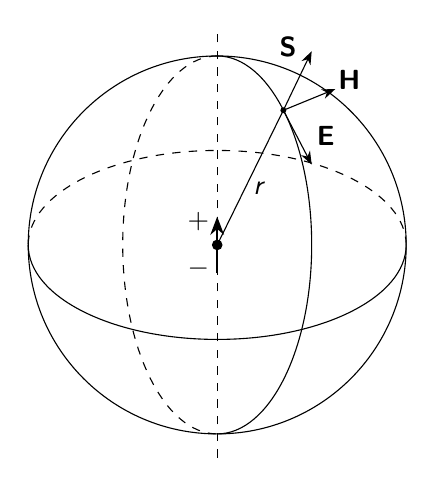
\begin{tikzpicture}[scale=0.6]
    %%Decartes_coordinate
    \draw[dashed] (0,-4.5) to (0,4.5);
    % \draw[-Stealth] (0,0) to (0,5);
    % \draw[-Stealth] (0,0) to (5,0);
    % \draw[-Stealth] (0,0) to (-4,-3);
    \draw[fill=black] (0,0) circle (0.1);
    
    % \draw 
    % (4.5,0) node[above]{$y$}
    % (0,4.5) node[left]{$z$}
    % (-3.6,-2.6) node[left]{$x$};
    %%Sphere_coordinate
    \draw (0,0) circle (4);
    \draw (0,4) arc(90:-90:2 and 4);
    \draw[dashed] (0,4) arc(90:270:2 and 4);
    \draw (-4,0) arc(180:360:4 and 2);
    \draw[dashed] (4,0) arc(0:180:4 and 2);
    %%projection
    \draw[fill=black] (1.4,2.85) circle (0.05);
    \draw (0,0) to (1.4,2.85);
    \draw 
    % (-0.3,-1.2) node{$\phi$}
    % (0.25,1.4) node{$\theta$}
    (0.9,1.2) node{$r$};
    %%unit vector
    \draw[-Stealth] (1.4,2.85) to (2,4.1);
    \draw[-Stealth] (1.4,2.85) to (2,1.7);
    \draw[-Stealth] (1.4,2.85) to (2.5,3.3);
    \draw
    (2.8,3.5) node{\(\mathbf{H}\)}
    (2.3,2.3) node{\(\mathbf{E}\)}
    (1.5,4.2) node{\(\mathbf{S}\)};
    %%antenna
    \draw[thick, -Stealth] (0,-0.6) to (0,0.6);
    \draw 
    (-0.4,-0.5) node{\( - \)}
    (-0.4,0.5) node{\( + \)}
    ;
    % \draw (-0.8,0.1) node{$I, L$};
\end{tikzpicture}

\end{document}